\documentclass[a4paper,11pt]{article}
\usepackage[T1]{fontenc}
\usepackage[utf8]{inputenc}
\usepackage[english]{babel}
\usepackage{graphicx}
\usepackage{microtype}
\usepackage[osf]{mathpazo}
\usepackage[x11names]{xcolor}
\usepackage[font=footnotesize,labelfont={bf}]{caption}
\usepackage{subfig}
\usepackage{listings}
    \lstset{language=[LaTeX]TeX,%
    basicstyle=\footnotesize\ttfamily,
    keywordstyle=\footnotesize\ttfamily\color{DodgerBlue1},
    commentstyle=\footnotesize\ttfamily\color{DarkOrchid1},
    showstringspaces=false,
    morecomment=[s][\footnotesize\ttfamily\color{brown!87!black}]\[ \],
    morecomment=[s][\footnotesize\ttfamily\color{brown!87!black}]< >,  
    texcsstyle=*\color{DodgerBlue1},
    morekeywords={invblock,opaqueblock,setalignment,dynalert,usetheme,alert,setinvopacity,
    setblockcolor,setbordercolor,setinnercolor,setoutercolor,settopcolor,setbottomcolor,
    setleftcolor,setrightcolor,fancyblock,vshadeblock,oshadeblock,DeclareOption,setbeamercolor},
    framerule=2pt,
    rulecolor=\color{DodgerBlue1},
    rulesep=4pt,
    framesep=5pt 
    }
%\lstdefinestyle{myslash}{%
%    literate={\textbackslash}{{\textcolor{DodgerBlue1}{\textbackslash}}}{1}%
%}
\usepackage[pdfpagelabels,plainpages=false,colorlinks=true,hyperindex=true,
							urlcolor=OrangeRed1,linkcolor=DodgerBlue1]{hyperref}

\newcommand*{\mcmd}[1]{\texttt{\{}\normalfont\texttt{#1}\texttt{\}}}
\newcommand*{\mbcmd}[1]{\texttt{[}\normalfont\texttt{#1}\texttt{]}}
\newcommand*{\meta}[1]{{\normalfont\ensuremath{\langle}\textit{#1}\ensuremath{\rangle}}}
\newcommand*{\marg}[1]{\texttt{\{\meta{#1}\}}}
\newcommand*{\sarg}[1]{\texttt{<\meta{#1}>}}
\newcommand*{\mbarg}[1]{\texttt{[\meta{#1}]}}
\newcommand*{\cs}[1]{\texttt{\char92#1}}

\renewcommand\labelitemi{\color{DodgerBlue1!60}$\bullet$} 
\renewcommand\labelitemii{\color{DodgerBlue1!60}$\circ$} 

\newcommand{\name}{\textsf{dynblocks}}
\newcommand{\version}{0.2b}
\newcommand{\versiondate}{187/09/2014}

\author{Claudio Fiandrino \\ \footnotesize{\href{mailto:claudio.fiandrino@gmail.com}{claudio.fiandrino@gmail.com}}}
\title{The \name{} package \footnote{This package has version number \textit{v}\version{} of \versiondate{}; it is released under and subject to the \href{http://www.latex-project.org/lppl/}{\LaTeX\ Project Public License (LPPL)}.}}

\begin{document}
\maketitle
\begin{abstract}
The \name{} package allows to fully customize blocks aspect and dimension inside a presentation.

The package originated from \href{http://tex.stackexchange.com/questions/53784/overlay-images-and-block-in-beamer}{this question} in \href{http://tex.stackexchange.com/}{TeX.SE}. The core functionalities of the package are based on \href{http://tex.stackexchange.com/questions/53784/overlay-images-and-block-in-beamer/53797#53797}{this answer}.
\end{abstract}

\tableofcontents

\section{Introduction}
The purpose of the package is to provide an instrument to customize several aspects of blocks (here called \emph{dynblocks}):
\begin{itemize}
\item the width;
\item the color
\begin{itemize}
\item of the background;
\item of the border;
\end{itemize}
\item the text:
\begin{itemize}
\item alignment;
\item opacity
\end{itemize}
\end{itemize}
Notice that \emph{dynblocks} defined by \name{} differ from usual beamer's blocks because no title is given.

The package has the following requirements:
\begin{itemize}
\item \textsf{TikZ};
\item \textsf{etoolbox};
\item \textsf{xparse}.
\end{itemize}

I would like to thank Enrico Gregorio for having pointed out an issue after the release of Ti\textit{k}Z 3.0.0 and \textsf{xparse} version 2014/08/25.

\section{Usage}
To load the package use as usual:  \cs{usepackage}\mbarg{options}\mcmd{dynblocks}.

The different options that can be adopted will be analysed in detail in section \ref{sec:options}.

\subsection{Basic usage}
Using the package in basic mode allows to define a block with:
\begin{itemize}
\item \emph{justified} alignment;
\item width equal to \cs{textwidth};
\item border color \cs{blue} and fill color \cs{blue!10}.
\end{itemize}
thanks to the command \cs{opaqueblock}\sarg{overlay spec}\mbarg{width}\marg{text}. Notice that \sarg{overlay spec} could be:
\begin{itemize}
\item a single number: \texttt{<1>};
\item multiple numbers separated by commas and delimited by braces: \texttt{<\{1,2,3\}>};
\item a single number followed by a dash: \texttt{<1->}.
\end{itemize}
Moreover, it is also possible to make it \emph{invisible}, that is to force colors to become \texttt{gray} by means of \cs{invblock}\sarg{overlay spec}. For example, the following code, generates the two frames shown in figures \ref{fig:basic1} and \ref{fig:basic2}.
\medskip
\begin{lstlisting}[frame=lines]
\documentclass{beamer}
\usepackage{dynblocks}

\usetheme{Luebeck}

\begin{document}
\begin{frame}{The frame title}
\begin{columns}[T]
 \begin{column}{0.4\textwidth}
  \begin{dynblock}
  \opaqueblock<1>[0.8\textwidth]{hello this is a dynamic block 
   with an itemize environment:
  \begin{itemize}
   \item hello
   \item hello again
  \end{itemize}
  } 
  \invblock<2->
  \end{dynblock}
 \end{column}
 \begin{column}{0.4\textwidth}
  \begin{dynblock}
  \opaqueblock<2>{hello this is another dynamic block}
  \end{dynblock}
 \end{column}
\end{columns}
\end{frame}

\end{document}
\end{lstlisting}

\begin{figure}[ht]
\centering
\subfloat[First frame]{
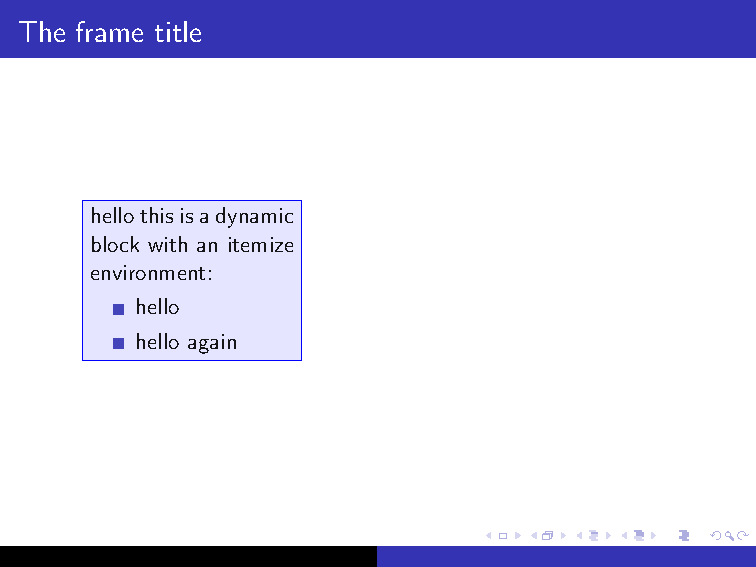
\includegraphics[scale=0.45]{./images/basic_1}
\label{fig:basic1}%
}
\hspace*{0.25cm}
\subfloat[Second frame]{
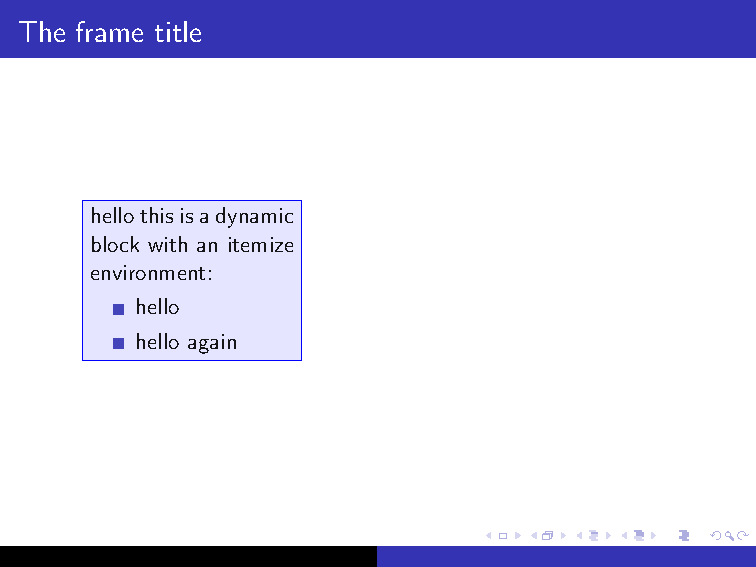
\includegraphics[scale=0.45]{./images/basic_2}
\label{fig:basic2}%
}
\caption{The basic example}
\end{figure}

In this example, it is possible to notice that the second \cs{opaqueblock} has no specified \texttt{width}; the default value is \cs{textwidth}, but if the block is placed inside a \emph{column} environment it automatically inherits the \texttt{width} given there. To set different values of \texttt{width}, it is necessary to specify the optional argument as did for the first \cs{opaqueblock} of the example.

The presence of an \cs{invblock} makes the first \cs{opaqueblock} invisible; this command needs to be placed immediately after an \cs{opaqueblock} because of two facts:
\begin{itemize}
\item it automatically inherits the \texttt{width} from the \cs{opaqueblock};
\item it automatically shows the text of the previous \cs{opaqueblock}.
\end{itemize}

Finally, both \cs{opaqueblock} and \cs{invblock} need to be placed inside a \texttt{dynblock} environment.

\subsection{Change text alignment}
Thanks to the command \cs{setalignment}\marg{text spec} the text alignment changes according to the \meta{text spec} (for all possibilities please refer to the pgfmanual section 17.4.3 -  version December 20, 2013).

Suppose, for instance, to modify the previous example in order to display the second block with center aligned text. The only change to do is:
\medskip
\begin{lstlisting}[frame=lines]
\begin{dynblock}
\setalignment{center}
\opaqueblock<2>{hello this is another dynamic block}
\end{dynblock}
\end{lstlisting}

and this will lead to figure \ref{fig:align}.

\begin{figure}[ht]
\centering
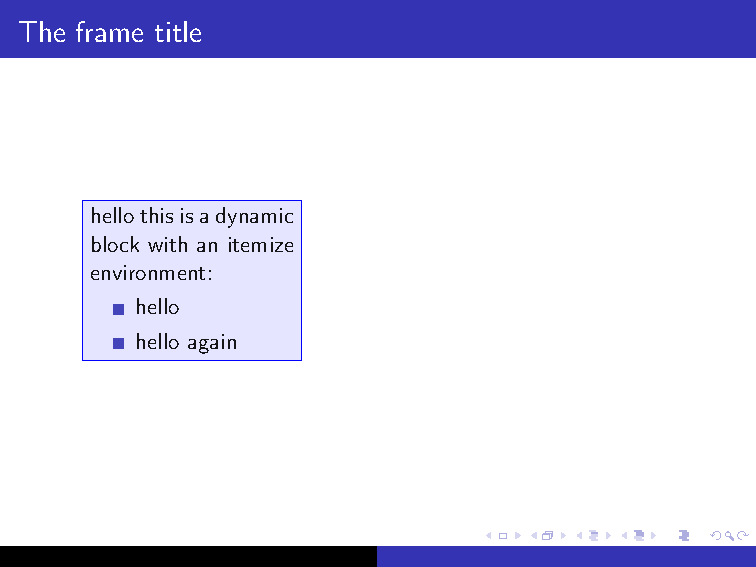
\includegraphics[scale=0.7]{./images/align}
\caption{Second frame with text center aligned for the second block}%
\label{fig:align}%
\end{figure}

Notice that the alignments can be local or global: if there is a definition in the preamble (global), all the \emph{dynblocks} will be set according to this definition. When the definition is set inside a group (a \emph{columns} environment or even simpler, the \emph{dynblock} environment), it affects only locally the \emph{dynblocks}. It is even possible set a global definition and then make local changes.

\subsection{Text opacity and word alert}
By default:
\begin{itemize}
\item \cs{opaqueblock}s have an opacity set to $0.9$;
\item \cs{invblock}s have an opacity set to $0.4$.
\end{itemize}
To change these values two commands have been introduced:
\begin{itemize}
\item \cs{setvisopacity}\marg{opacity spec};
\item \cs{setinvopacity}\marg{opacity spec};
\end{itemize}
where \meta{opacity spec} is a value in the interval $[0 \, , \, 1]$. Also these commands can be set locally or in a global fashion in the preamble. 

Due to the opacity, the usual \cs{alert} command is not more useful with \cs{invblock}s. The package provides a method to alert a word even in this case. The command to be used is \cs{dynalert}\sarg{overlay spec}\marg{text}. Note that with the proper usage of \meta{overlay spec}, \cs{dynalert} must not fall inside a \cs{opaqueblock}. This is a limitation because the purpose for which it has been developed is different. 

Assume, for example, to modify the reference example such that the opacity of \cs{invblock} will be set to $0.1$; furthermore, for the first block, the word ``\emph{itemize}'' will be alerted with \cs{alert}, while ``\emph{dynamic block}'' with \cs{dynalert} and for the second block (that does not have the correspondent \cs{invblock}) it is shown what happens with a wrong  usage of \cs{dynalert}. The code is:
\medskip
\begin{lstlisting}[frame=lines]
\documentclass{beamer}
\usepackage{dynblocks}

\usetheme{Luebeck}
\setinvopacity{0.1}

\begin{document}
\begin{frame}{The frame title}
\begin{columns}[T]
\begin{column}{0.4\textwidth}
\begin{dynblock}
\opaqueblock<1>[0.8\textwidth]{hello this is a 
 \dynalert<2>{dynamic block} with an \alert<1,2>{itemize} 
  environment:
\begin{itemize}
\item hello
\item hello again
\end{itemize}
}
\invblock<2->
\end{dynblock}
\end{column}
\begin{column}{0.4\textwidth}
\begin{dynblock}
\opaqueblock<2>{hello this is another 
 \dynalert<2>{dynamic} block}
\end{dynblock}
\end{column}
\end{columns}
\end{frame}

\end{document}
\end{lstlisting}

\begin{figure}[ht]
\centering
\subfloat[First frame]{
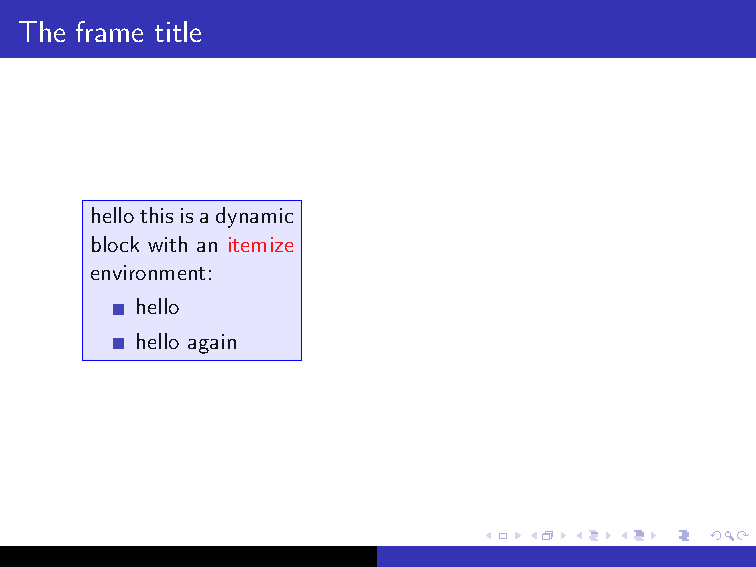
\includegraphics[scale=0.45]{./images/alert_1}
\label{fig:alert1}%
}
\hspace*{0.1cm}
\subfloat[Second frame]{
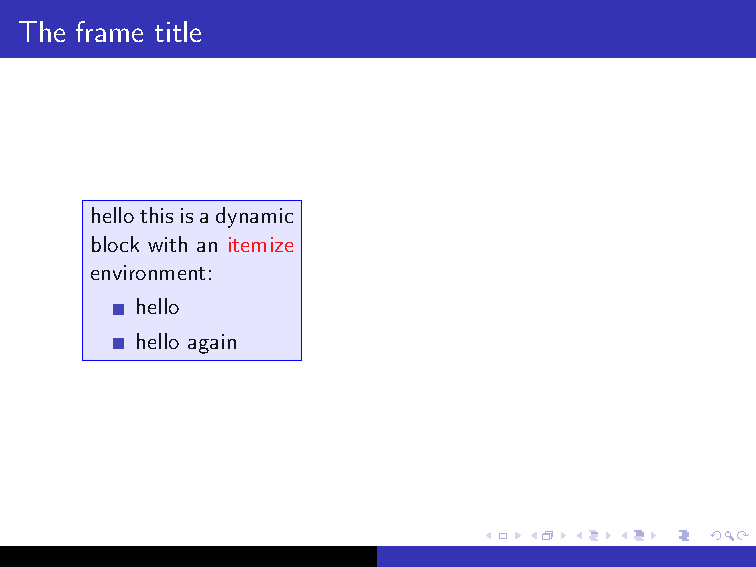
\includegraphics[scale=0.45]{./images/alert_2}
\label{fig:alert2}%
}
\caption{Example with different opacity and alerts}
\end{figure}

As it is possible to see from figures \ref{fig:alert1} and \ref{fig:alert2}, the usual \cs{alert}, when used inside an \cs{invblock}, is set with the opacity of the block while the proper \cs{dynalert} no. Anyway, a wrong usage of \cs{dynalert} lead to the output shown in figure \ref{fig:alert2}: the subsequent text of the alerted word is set with the opacity of an \cs{invblock}. 

The suggested use, in conclusion, is:
\begin{itemize}
\item \cs{alert} with \meta{overlay spec} equal specified in the related \cs{opaqueblock};
\item \cs{dynalert} to highlight words inside an \cs{invblock};
\item never do something like: \cs{dynalert}\texttt{<1,2>}\mcmd{word} if the \cs{opaqueblock} is shown in \meta{overlay spec}$=1$ and the \cs{invblock} in \meta{overlay spec}$=2$. 
\end{itemize}

To change colors:
\begin{itemize}
\item for \cs{alert} the usual Beamer command works:\\ \cs{setbeamercolor}\mcmd{alerted text}\marg{color spec};
\item for \cs{dynalert} a different command has been introduced to differentiate them from standard Beamer's alerts: \cs{setwordscolor}\marg{color}; the default value is set to \textit{blue}.
\end{itemize}

\section{Options and advanced examples}\label{sec:options}
In this section the package's options are introduced with examples. They allow to customize more deeply the aspect of \emph{dynblocks}:
\begin{itemize}
\item adding the shadow and the rounded corners (subsection \ref{subse:shrc});
\item customizing the fill color (subsection \ref{subse:cfill});
\item adapting the fill color to the current Beamer theme used (subsection \ref{subse:cadapt}).
\end{itemize}

\subsection{The shadow and the rounded corners}\label{subse:shrc}
To load:
\begin{itemize}
\item the shadow option use: \cs{usepackage}\mbcmd{shadow}\mcmd{dynblocks}; it is possible to set the \emph{shadow opacity} by means of the following command: \cs{setshadowopacity}\marg{opacity spec} (default value $0.4$); 
\item the option to have rounded corners for \emph{dynblocks} use: \\ \cs{usepackage}\mbcmd{roundedcorners}\mcmd{dynblocks}.
\end{itemize}

For example:
\begin{lstlisting}[frame=lines]
\documentclass{beamer}
\usepackage[shadow,roundedcorners]{dynblocks}

\usetheme{Luebeck}

\begin{document}
\begin{frame}{The frame title}
\begin{columns}[T]
\begin{column}{0.4\textwidth}
\begin{dynblock}
\opaqueblock<1>[0.8\textwidth]{hello this is a 
 \dynalert<2>{dynamic block}  with an 
 \alert<1,2>{itemize} environment:
\begin{itemize}
\item hello
\item hello again
\end{itemize}
}
\invblock<2->
\end{dynblock}
\end{column}
\begin{column}{0.4\textwidth}
\begin{dynblock}
\setalignment{center}
\opaqueblock<2>{hello this is another dynamic block}
\end{dynblock}
\end{column}
\end{columns}
\end{frame}

\end{document}
\end{lstlisting}
allows to get the frames shown in figures \ref{fig:shdrndc1} and \ref{fig:shdrndc2}.

\begin{figure}[ht]
\centering
\subfloat[First frame]{
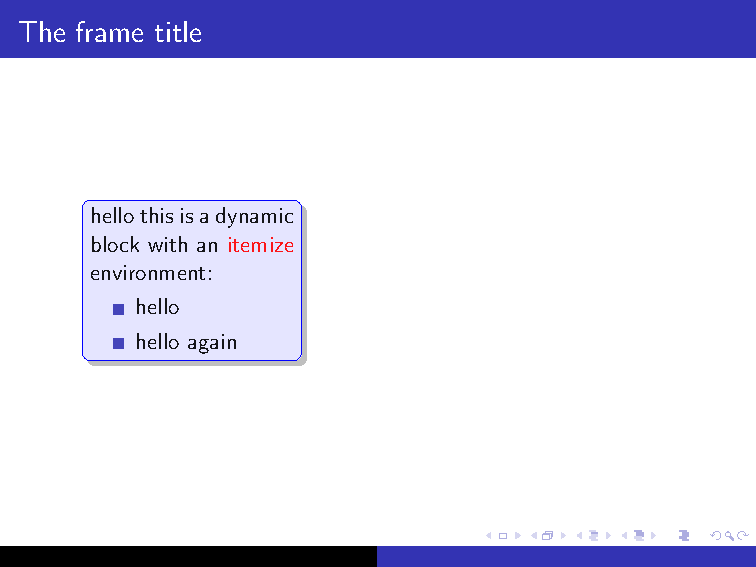
\includegraphics[scale=0.45]{./images/shdrndc_1}
\label{fig:shdrndc1}%
}
\hspace*{0.1cm}
\subfloat[Second frame]{
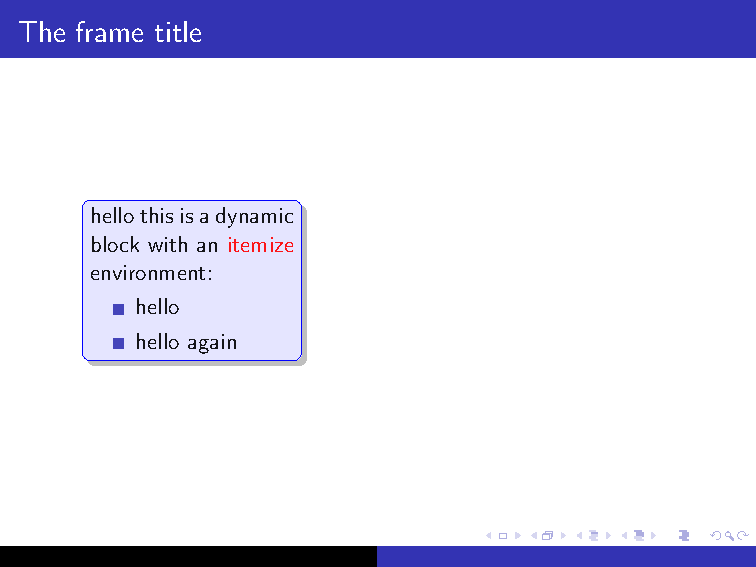
\includegraphics[scale=0.45]{./images/shdrndc_2}
\label{fig:shdrndc2}%
}
\caption{Example with \texttt{shadow} and \texttt{roundedcorners} options}
\end{figure}

\subsection{Customized fill colors}\label{subse:cfill}
By activating this option it is possible to fully customize the \emph{dynblocks} colors  because several command become available:
\begin{itemize}
\item \cs{setblockcolor}\marg{color spec} and \cs{setbordercolor}\marg{color spec} for the \cs{opaqueblock}s (default values are \textit{blue!10} and \textit{blue} respectively);
\item \cs{setinnercolor}\marg{color spec} and \cs{setoutercolor}\marg{color spec} for the \cs{fancyblock}s (default values are \textit{white} and \textit{blue!10} respectively);
\item \cs{settopcolor}\marg{color spec} and \cs{setbottomcolor}\marg{color spec} for the \cs{vshadeblock}s (default values are \textit{white} and \textit{blue!10} respectively);
\item \cs{setleftcolor}\marg{color spec} and \cs{setrightcolor}\marg{color spec} for the \cs{oshadeblock}s (default values are \textit{white} and \textit{blue!10} respectively).
\end{itemize}
Similarly to the \texttt{shadow} and the \texttt{roundedcorners} options, to load the \texttt{customcolors} option use \cs{usepackage}\mbcmd{customcolors}\mcmd{dynblocks}.

In the following example, all \emph{dynblocks} types are used and it is possible to see how local and global setting work.

\begin{lstlisting}[frame=lines]
\documentclass{beamer}
\usepackage[shadow, roundedcorners,customcolors]{dynblocks}
% some global settings
\setblockcolor{red!10}
\setbordercolor{red}
\setbottomcolor{orange!40}
\setrightcolor{orange!40}

\usetheme{Luebeck}

\begin{document}
\begin{frame}{The frame title}
\begin{columns}[T]
\begin{column}{0.4\textwidth}
\begin{dynblock}
\opaqueblock<1>[0.8\textwidth]{hello this is a 
 \dynalert<2>{dynamic block} with an 
 \alert<1,2>{itemize} environment:
\begin{itemize}
\item hello
\item hello again
\end{itemize}
}
\invblock<2->
\end{dynblock}
\end{column}
\begin{column}{0.4\textwidth}
\setalignment{center}
\begin{dynblock}
% default settings since no
% \setinnercolor or \setoutercolor
% are there
\fancyblock<2>{hello this is another dynamic block}
\invblock<3->
\end{dynblock}
\\[2ex]
\setbordercolor{orange} % local definition 
% that overwrites the global one
\begin{dynblock}
\vshadeblock<3>{replica: hello this a another dynamic block}
\invblock<4->
\end{dynblock}
\\[2ex]
\begin{dynblock}
\oshadeblock<4>{replica 2: hello this a another dynamic block}
\end{dynblock}
\end{column}
\end{columns}
\end{frame}

\end{document}
\end{lstlisting}

The four frames obtained by this example are shown in figures \ref{fig:custcol1}, \ref{fig:custcol2}, \ref{fig:custcol3} and \ref{fig:custcol4}; more in detail:
\begin{itemize}
\item an example of \cs{opaqueblock} customization through \cs{setblockcolor} and \cs{setbordercolor} could be seen in figure \ref{fig:custcol1};
\item an example of \cs{fancyblock} with default settings could be seen in figure \ref{fig:custcol2} (notice that it inherits the \texttt{bordercolor} from the global setting);
\item an example of \cs{vshadeblock} with customization of \cs{setbottomcolor} and locally \cs{setbordercolor} (\cs{settopcolor} at default value) could be seen in figure \ref{fig:custcol3};
\item finally, an example of \cs{oshadeblock} with \cs{setrightcolor} and local \cs{setbordercolor} customization (\cs{settopcolor} at default value) could be seen in figure \ref{fig:custcol4}.
\end{itemize}

\begin{figure}[ht]
\centering
\subfloat[First frame]{
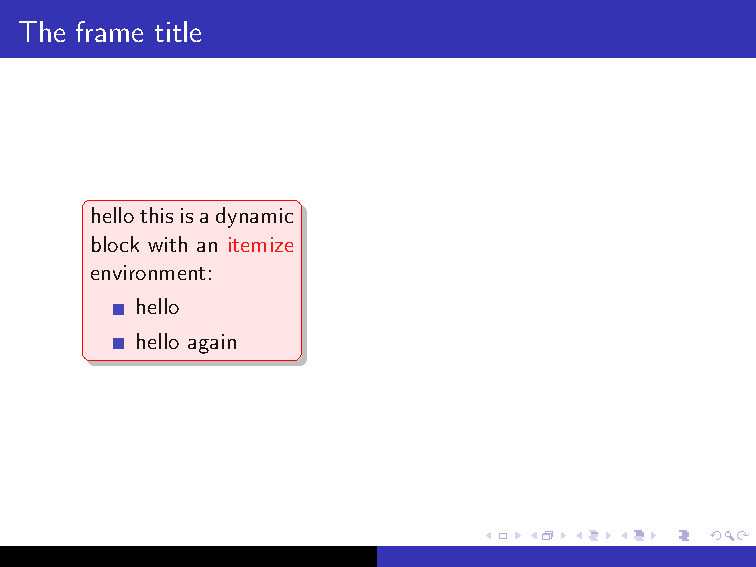
\includegraphics[scale=0.45]{./images/custcol_1}
\label{fig:custcol1}%
}
\hspace*{0.25cm}
\subfloat[Second frame]{
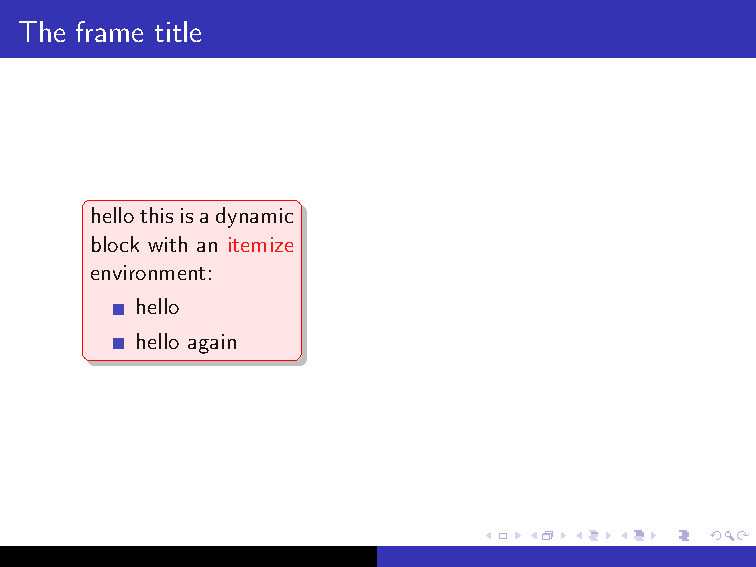
\includegraphics[scale=0.45]{./images/custcol_2}
\label{fig:custcol2}%
}
\\
\subfloat[Third frame]{
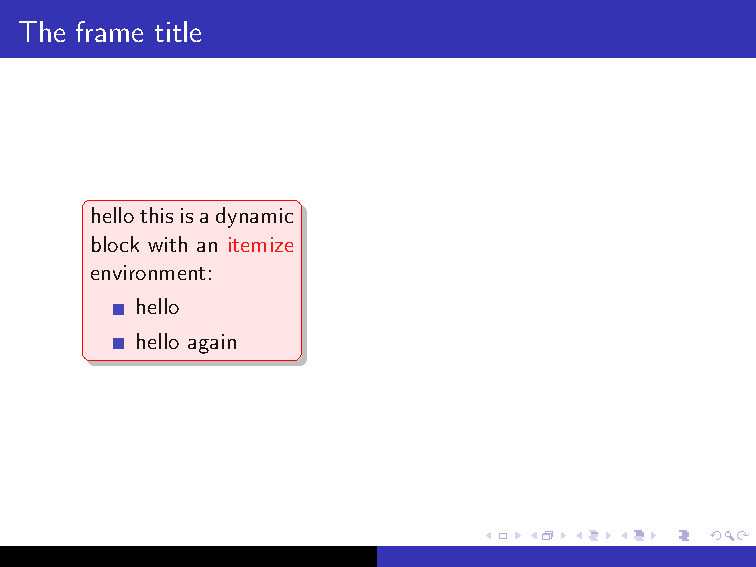
\includegraphics[scale=0.45]{./images/custcol_3}
\label{fig:custcol3}%
}
\hspace*{0.25cm}
\subfloat[Fourth frame]{
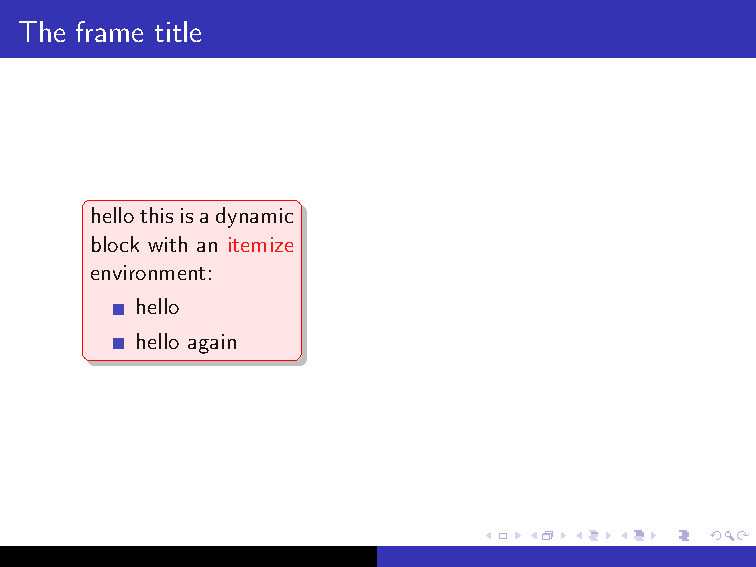
\includegraphics[scale=0.45]{./images/custcol_4}
\label{fig:custcol4}%
}
\caption{Example with \texttt{customcolor} option and all \emph{dynblocks} types}
\end{figure}

\subsection{Color adaptation to the Beamer theme}\label{subse:cadapt}
The purpose of this option is to use the Beamer's color of the theme currently adopted; as it will be possible to see, the \texttt{getthemecolors} option should be used with particular care. To load the option there is the usual \cs{usepackage}\mbcmd{getthemecolors}\mcmd{dynblocks}.

This option is defined inside the package as:
\begin{lstlisting}[frame=lines]
\DeclareOption{getthemecolors}{
% redefinition opaqueblock
\renewcommand{\thecol}{structure.fg!10}
\renewcommand{\thebordercol}{structure.fg}
% redefinition fancyblock
\def\@setinnercolor{white}
\def\@setoutercolor{structure.fg!10}
% redefinition vshadeblock
\def\@settopcolor{white}
\def\@setbottomcolor{structure.fg!10}
% redefinition oshadeblock
\def\@setleftcolor{white}
\def\@setrightcolor{structure.fg!10}
}
\end{lstlisting}
thus it works properly if the current \texttt{beamercolortheme} set the \emph{structure} definition.

For example:
\begin{lstlisting}[frame=lines]
\documentclass{beamer}
\usepackage[shadow, roundedcorners,getthemecolors,
   customcolors]{dynblocks}

\usetheme{CambridgeUS}

\begin{document}
\begin{frame}{The frame title}
\begin{columns}[T]
\begin{column}{0.4\textwidth}
\begin{dynblock}
\opaqueblock<1>[0.8\textwidth]{hello this is a 
\dynalert<2>{dynamic block} with an 
\alert<1,2>{itemize} environment:
\begin{itemize}
\item hello
\item hello again
\end{itemize}
}
\invblock<2->
\end{dynblock}
\end{column}
\begin{column}{0.4\textwidth}
\setalignment{center}
\begin{dynblock}
\opaqueblock<2>{hello this is another dynamic block}
\end{dynblock}
\end{column}
\end{columns}
\end{frame}

\end{document}
\end{lstlisting}
will lead to figures \ref{fig:cmbx1} and \ref{fig:cmbx2}.
\begin{figure}[ht]
\centering
\subfloat[First frame]{
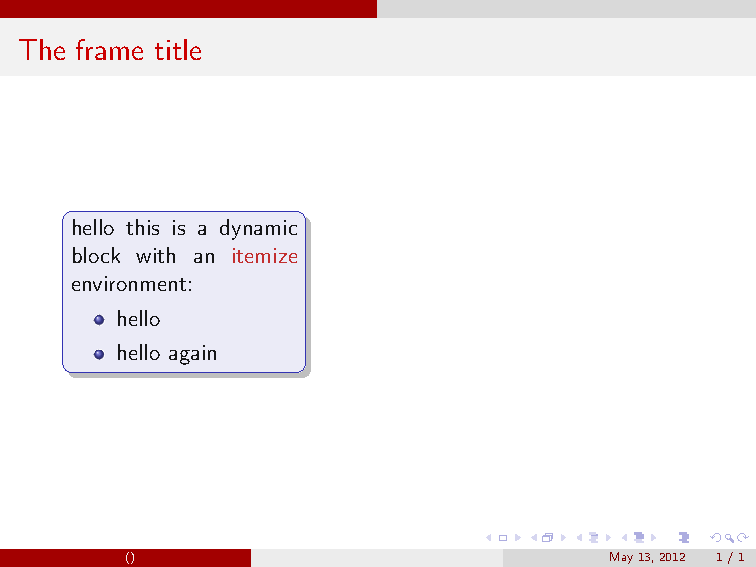
\includegraphics[scale=0.45]{./images/cmbx_1}
\label{fig:cmbx1}%
}
\hspace*{0.1cm}
\subfloat[Second frame]{
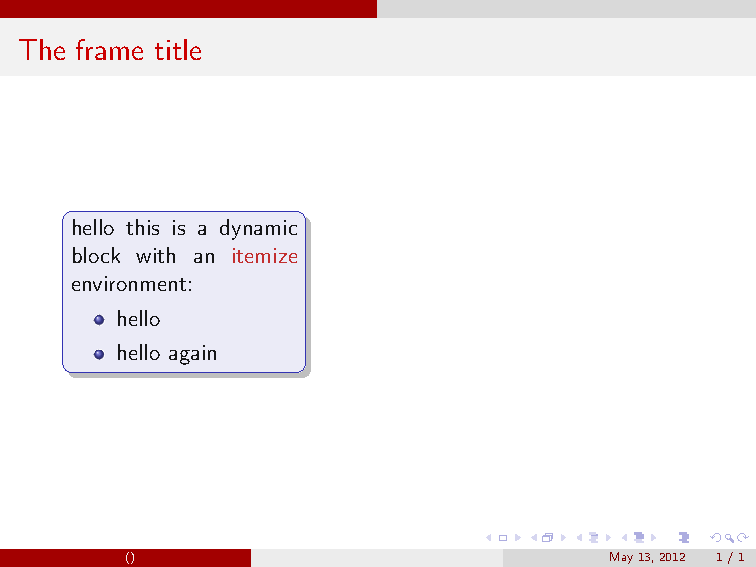
\includegraphics[scale=0.45]{./images/cmbx_2}
\label{fig:cmbx2}%
}
\caption{Example with a theme that does not define structure color}
\end{figure}

The result can be improved in the following way:
\begin{lstlisting}[frame=lines]
\documentclass{beamer}
\usepackage[shadow, roundedcorners,getthemecolors,
   customcolors]{dynblocks}

\usetheme{CambridgeUS}
% definition of structure
\setbeamercolor*{structure}{parent=palette primary}

\begin{document}
\begin{frame}{The frame title}
\begin{columns}[T]
\begin{column}{0.4\textwidth}
\begin{dynblock}
\opaqueblock<1>[0.8\textwidth]{hello this is a 
\dynalert<2>{dynamic block} with an 
\alert<1,2>{itemize} environment:
\begin{itemize}
\item hello
\item hello again
\end{itemize}
}
\invblock<2->
\end{dynblock}
\end{column}
\begin{column}{0.4\textwidth}
\setalignment{center}
\begin{dynblock}
\opaqueblock<2>{hello this is another dynamic block}
\end{dynblock}
\end{column}
\end{columns}
\end{frame}

\end{document}
\end{lstlisting}
obtaining as result the frames shown in figures \ref{fig:cmby1} and \ref{fig:cmby2}.

\begin{figure}[ht]
\centering
\subfloat[First frame]{
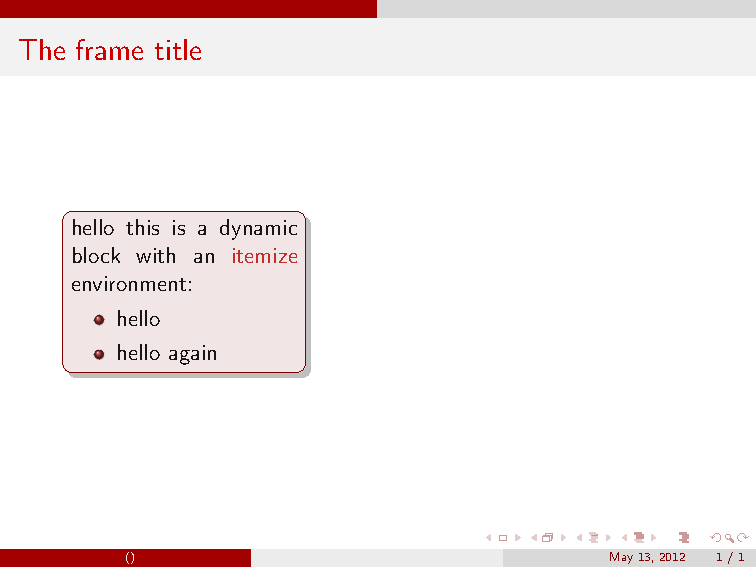
\includegraphics[scale=0.45]{./images/cmby_1}
\label{fig:cmby1}%
}
\hspace*{0.1cm}
\subfloat[Second frame]{
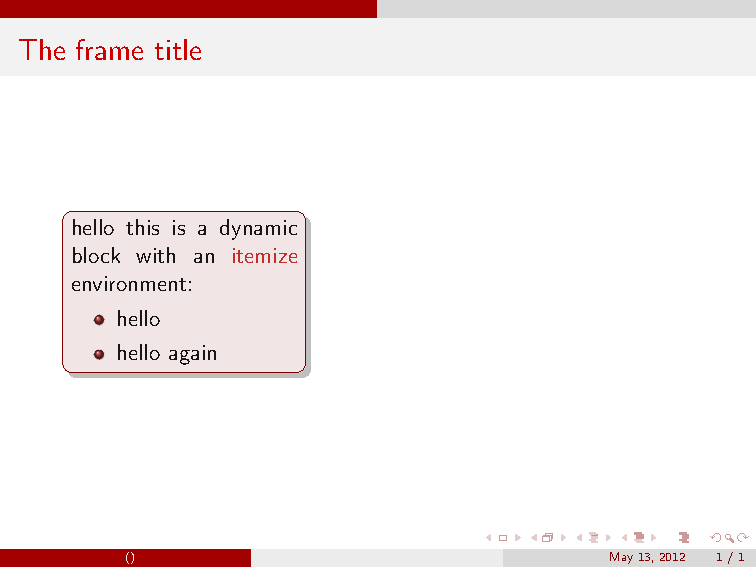
\includegraphics[scale=0.45]{./images/cmby_2}
\label{fig:cmby2}%
}
\caption{Example of a theme with a posteriori structure color definition}
\end{figure}


Here is another example:
\begin{lstlisting}[frame=lines]
\documentclass{beamer}
\usepackage[getthemecolors]{dynblocks}

\usetheme{EastLansing}
\setbeamercolor*{structure}{parent=palette primary}

\begin{document}
\begin{frame}{The frame title}
\begin{dynblock}
\opaqueblock<1>{hello this is a 
dynamic block with an 
itemize environment:
\begin{itemize}
\item hello
\item hello again
\end{itemize}
}
\end{dynblock}
\end{frame}

\end{document}
\end{lstlisting}
with the final output shown in figure \ref{fig:estl}.

\begin{figure}[ht]
\centering
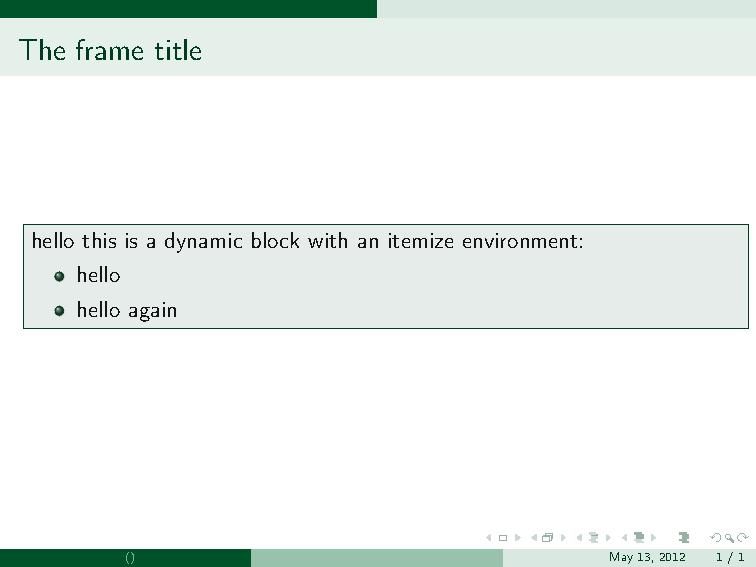
\includegraphics[scale=0.7]{./images/estl}
\caption{Second example of a theme with a posteriori structure color definition}%
\label{fig:estl}%
\end{figure}

The decision of adopting \emph{structure} as reference is due to the fact that this parameter is one of the most relevant while customizing a Beamer theme. In the following example, it is shown a color customization of the Szeged theme and a particular effect that can be realized thanks to multiple \emph{dynblocks} inside the same \texttt{dynblock} environment:
\begin{lstlisting}[frame=lines]
\documentclass{beamer}
\usepackage[getthemecolors,roundedcorners,shadow]{dynblocks}

\usetheme{Szeged}
\setbeamercolor{structure}{bg=red!20,fg=red}

\begin{document}


\begin{frame}{A title}
\begin{center}
\begin{dynblock}
\opaqueblock<1>[0.6\textwidth]{hello this is a dynamic block
 with an itemize environment:
\begin{itemize}
\item hello
\item hello again
\end{itemize}
}
\invblock<2->
\setalignment{center}
\opaqueblock<2>{hello this is another dynamic block}
\end{dynblock}
\end{center}
\end{frame}

\end{document}
\end{lstlisting}
The two frames obtained as outcome are shown in figures \ref{fig:szeg1} and \ref{fig:szeg2}.
\begin{figure}
\centering
\subfloat[First frame]{
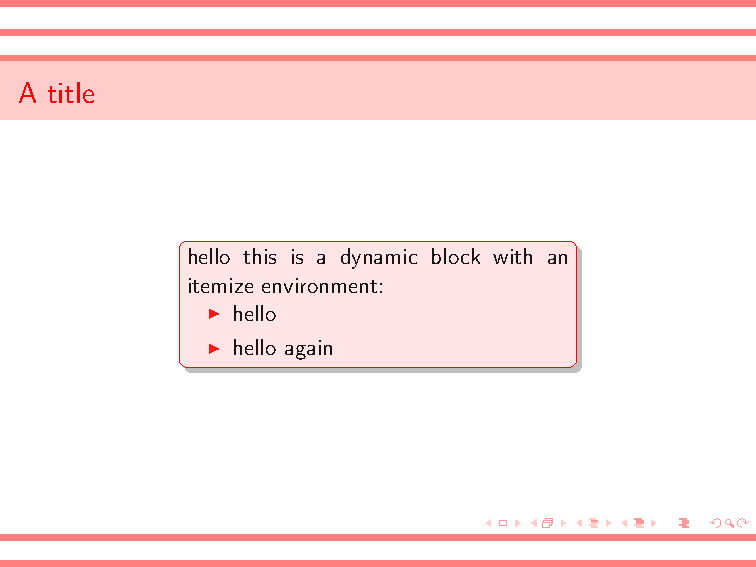
\includegraphics[scale=0.45]{./images/szeg_1}
\label{fig:szeg1}%
}
\hspace*{0.1cm}
\subfloat[Second frame]{
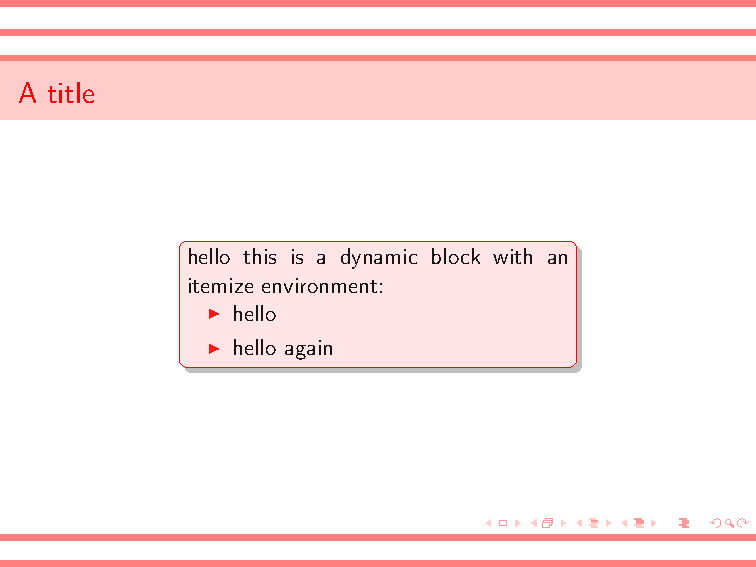
\includegraphics[scale=0.45]{./images/szeg_2}
\label{fig:szeg2}%
}
\caption{Example of a customized theme}
\end{figure}

Note that the \texttt{getthemecolors} option has some drawbacks when it is used with particular Beamer color themes like:
\begin{itemize}
\item albatross;
\item beetle.
\end{itemize}


\end{document}

